\usepackage{amsmath}

% !Mode:: "TeX:UTF-8"
% Author: Zhengxi Tian
% Email: zhengxi.tian@hotmail.com

\chapter{相关工作}\label{ch:related_work}
% ------------------ Models ------------------ %
\section{生成式模型}\label{sec:generative_model}
\subsection{定义}\label{subsec:definition}
一个生成式模型定义了给定输入序列$X = x_1, x_2, \cdots, x_n$,
任意输出序列$Y = y_1, y_2, \cdots, y_m$的条件概率:
\begin{align}
    p(Y|X) = P(y_1, y_2, \cdots, y_m|x_1, x_2, \cdots, x_n)
    \label{eqn:generative_conditional_probability}
\end{align}
% Sane way to do |S|:
% https://tex.stackexchange.com/questions/43008/absolute-value-symbols

模型的训练目标就是在数据集$S$上最大化给定$X$,$Y$的对数概率(Log Probability):
\begin{align}
    \mathit{L} = \frac{1}{\left |S| \right}
    \sum_{(Y, X) \in S} \log p(Y|X)
\end{align}
从定义上看,语言模型\upcite{NNLM,RNNLM}(Language Model)和编解码器(Encoder-Decoder)都属于生成式模型,
因为它们都定义了条件概率$p(Y|X)$。

% -- RNN -- %
生成式模型需要把一个长度可变的序列$X$映射到另一个长度可变的序列$Y$,且$X$和$Y$的长度可以不相等。
循环神经网络(RNN)为这个问题提供了自然的解决方案。
RNN的基本思想是:序列由有序的元素组成,每一个时刻(Time Step)输入一个元素,同时更新内部的隐藏状态(Hidden State),然后输出一个元素。
如图~\ref{fig:RNN_unrolled}\footnote{http://colah.github.io/posts/2015-08-Understanding-LSTMs/}~所示,
在时间轴上展开的RNN和一般的前馈神经网络(Feed Forward Neural Networks)很像,不过每一个时刻的权重矩阵都是共享的。
这个共享的权重矩阵$A$又被称为循环矩阵(Recurrent Matrix),
它的作用是对输入序列进行某种保持顺序信息的编码。

\begin{figure}[H]
    \centering
    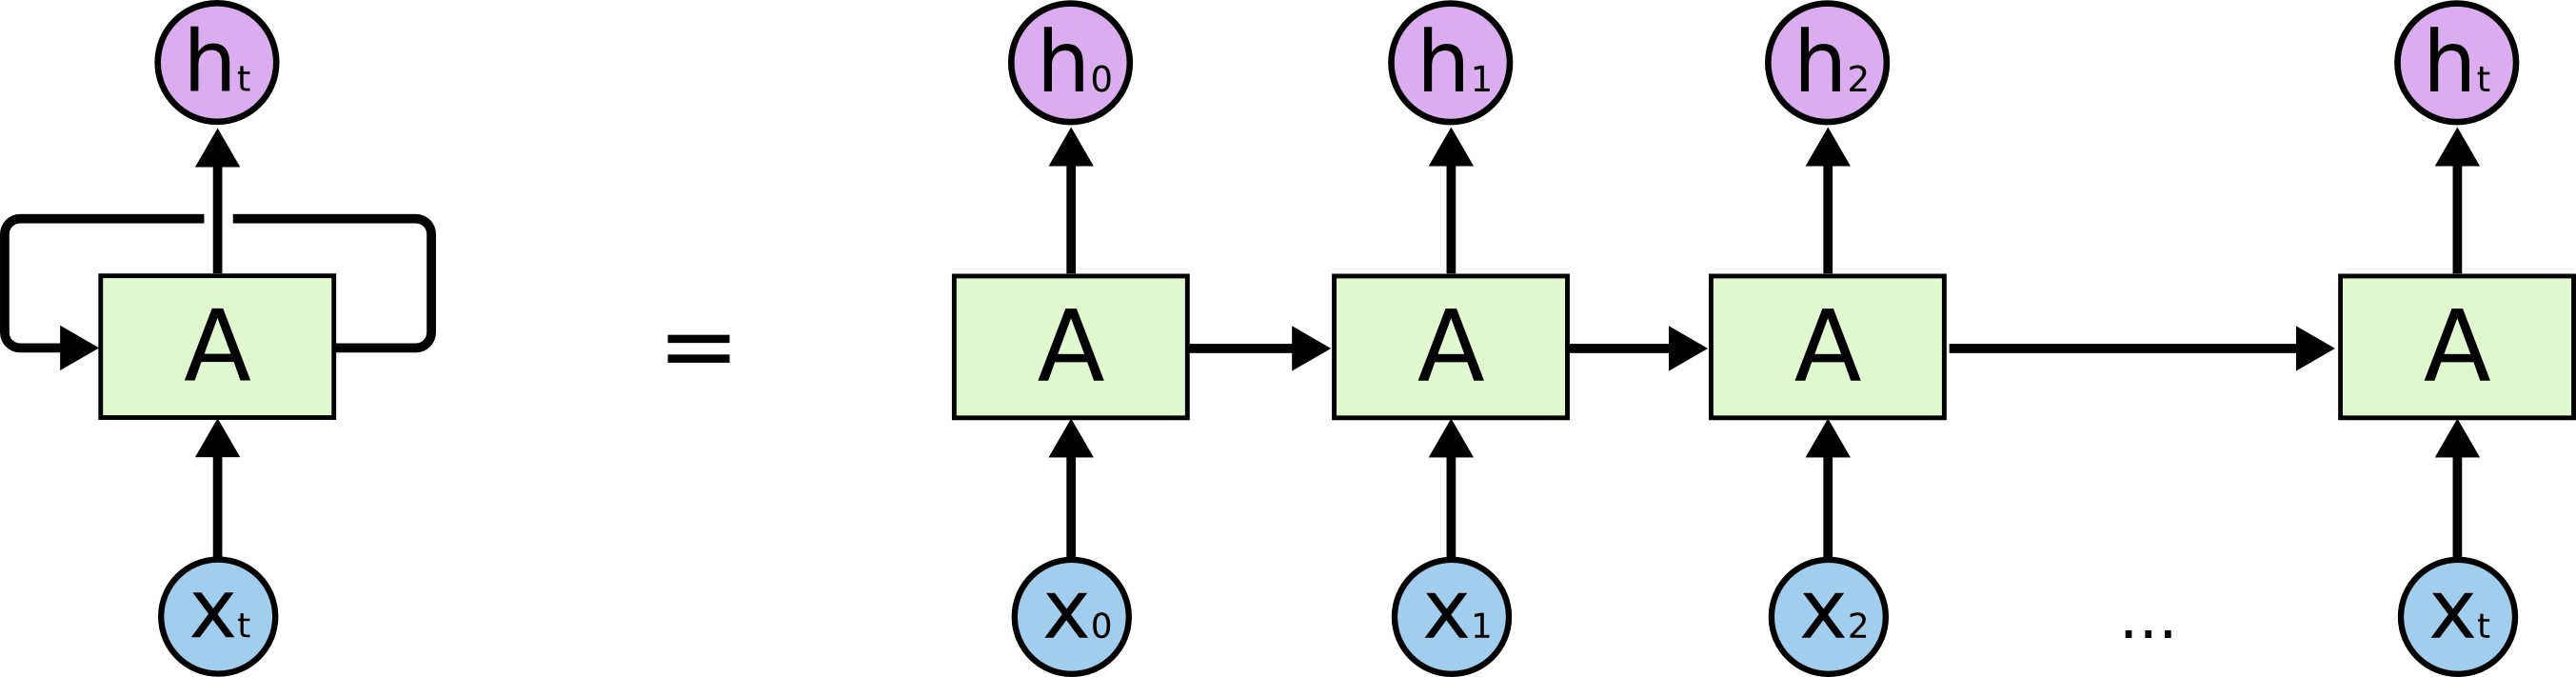
\includegraphics[width=0.6\textwidth]{figure/RNN-unrolled.png}
    \caption{在时间轴上展开的RNN}
    \label{fig:RNN_unrolled}
\end{figure}

% ------------------ RNN types ------------------ %
根据是否使用了某种门单元,RNN可分为普通RNN\upcite{RNNLM},
LSTM\upcite{LSTM}和GRU\upcite{GRU}。
根据是否对反向序列(Reversed Sequence)编码,
RNN可分为单向RNN(Unidirectional RNN)
和双向RNN(Bidirectional RNN)\upcite{BiRNN}。
由于普通RNN受到梯度消失的影响,目前学界普遍采用LSTM或者GRU;
尽管后者受到梯度爆炸的影响,但是可以通过梯度剪裁(Gradient~Clipping)
\upcite{GoogleChatbot}解决。
此外,多层RNN组成的深度循环神经网络比单层RNN有更好的性能\upcite{GoogleChatbot}。

\subsection{RNN语言模型}\label{subsec:RNNLM}
% ---------------- RNNLM ------------------ %
RNN语言模型通过循环神经网络估计给定序列$X=x_1, x_2, \cdots, x_n$的概率分布:
\begin{align}
    p(X) = \prod_{i=1}^{n} p(x_i|x_1, x_2, \cdots, x_{i-1})
    \label{eqn:language_model_probability} \\
    p(x_i = w|x_1, x_2, \cdots, x_{i-1}) = \frac{\exp{o_{tw}}}{\sum_{v=1}^V \exp{o_{tv}}}
    \label{eqn:language_model_estimation}
\end{align}

$o_t$是RNN的在$t$时刻的输出向量,$V$是词汇表的大小,
RNN语言模型\footnote{为了简洁起见,我们描述了不使用任何门单元的RNN。LSTM和GRU有着更复杂的数学表达式。}通过如下公式计算出$o_t$:
\begin{align}
    o_i &= h_i^T W_{out} \\
    h_i &= \sigma \left( x_i^T W_{in} + h_{i-1}^T W_{hh} \right)
\end{align}

$W_{in}$是输入矩阵,$W_{out}$是输出矩阵,$W_{hh}$是循环矩阵,
$\sigma$是激活函数。
RNN语言模型在训练时最大化训练集上的句子的对数概率:
\begin{align}
    \mathit{L(X)} = \sum_{i=1}^n \log p(x_i|x_1, x_2, \cdots, x_{i-1})
\end{align}

在解码时,RNN语言模型通过预测下一个单词,从一个全零的初态开始生成句子。

\subsection{Seq2Seq框架}\label{subsec:Seq2Seq}
% ------------------ Seq2Seq ------------------ %
如图~\ref{fig:Seq2Seq}~所示,
Seq2Seq框架使用两个有着独立参数的RNN分别作为编码器和解码器。
首先,编码器把输入序列$X$编码成一个定长向量$v$。
该向量又称为思考向量(Though Vector),
是编码器的最后一个隐藏状态(Last Hidden State)。
接着,解码器以$v$为初始隐藏状态(Initial Hidden State),
像RNN语言模型一样生成输出序列。
\begin{figure}[H]
    \centering
    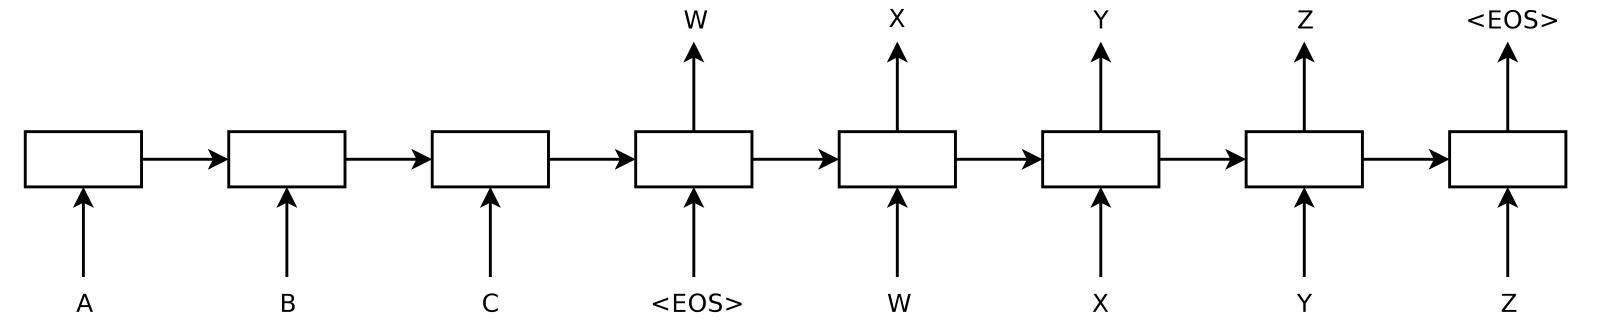
\includegraphics[width=0.8\textwidth]{figure/Seq2Seq.png}
    \caption{Seq2Seq框架图\upcite{Seq2Seq}}
    \label{fig:Seq2Seq}
\end{figure}

通过先把输入序列$X$变换成某种压缩编码$v$,
再把$v$还原为另一个序列$Y$,
Seq2Seq把公式~\ref{eqn:generative_conditional_probability}~作了如下转化:
\begin{align}
    h_i &= f(x_i ,h_{i-1}) \\
    v &= h_n \\
    p(y_1, y_2, \cdots, y_m|x_1, x_2, \cdots, x_n) &=
    \prod_{i=1}^m p(y_i|v, y_1, y_2, \cdots, y_{i-1})
\end{align}

$h_n$是编码器的最后一个隐藏状态, $f$是编码器采用的门单元函数。
编码器和解码器以同一个目标函数同时训练。

为了更好的处理长序列,
Seq2Seq一般引入注意力机制(Attention Mechanism)
\upcite{JointTransAlign,EffectiveAttention},
使输入序列的信息不必全部通过固定长度的向量$v$传递。
该机制使解码器能自动关注和当前输出最相关的输入部分,
实现输入序列与输出序列的对自动对齐(Automatic Alignment)。


\subsection{多层编解码器}\label{subsec:hierarchical_rnn}
多层编解码器(Hierarchical Recurrent Encoder-Decoder,HRED)\upcite{hred-qs}是一种能利用多轮对话结构的生成式模型。
它把一个对话看做一个两层序列结构:一个对话$D$由$M$个句子组成,每个句子由$N_m$个单词组成:
\begin{align}
    D &= \{ U_1, \cdots, U_M \} \\
    U_m &= \{ w_{m, 1}, \cdots, w_{m, N_m} \}
\end{align}

HRED由三个RNN组成:一个编码RNN(Encoder RNN)负责把每一个句子编码成一个固定长度的向量,称为句子向量(Utterance Vector);
一个上下文RNN(Context RNN)负责迭代的处理句子向量,
把直到并且包括当前轮$m$的所有轮的句子$U_1, \cdots, U_m$编码成一个对话向量(Dialogue Vector);
最后,一个解码RNN(Decoder RNN)负责以对话向量为条件,生成对话的下一个句子$U_{m+1}$。
三个RNN的协作关系如~图\ref{fig:HRED_computation_graph}~所示。
本质上,HRED通过把对话分解为句子的序列,
把句子分解为单词的序列,估计了一个对话$D$的概率$P_{\theta}(D)$:
\begin{align}
    P_{\theta}(D) &= P_{\theta}(U_1, \cdots, U_M) \\
    &= \prod_{m=1}^M P_{\theta}(U_m|U_{<m}) \\
    &= \prod_{m=1}^M \prod_{n=1}^{N_m} P_{\theta}(
    w_{m, n} |w_{m, <n}, U_{<m}
    )
\end{align}

$\theta$是HRED模型的参数,
$U_{<m}$表示$U_m$之前的句子序列:
$U_{<m} = \{ U_1, \cdots, U_{m-1} \}$,
$w_{m, <n}$表示第$m$个句子的第$n$个单词之前的单词序列:
$w_{m, <n} = \{ w_{m, 1}, \cdots, w_{m, n-1} \}$。

\begin{figure}[H]
    \centering
    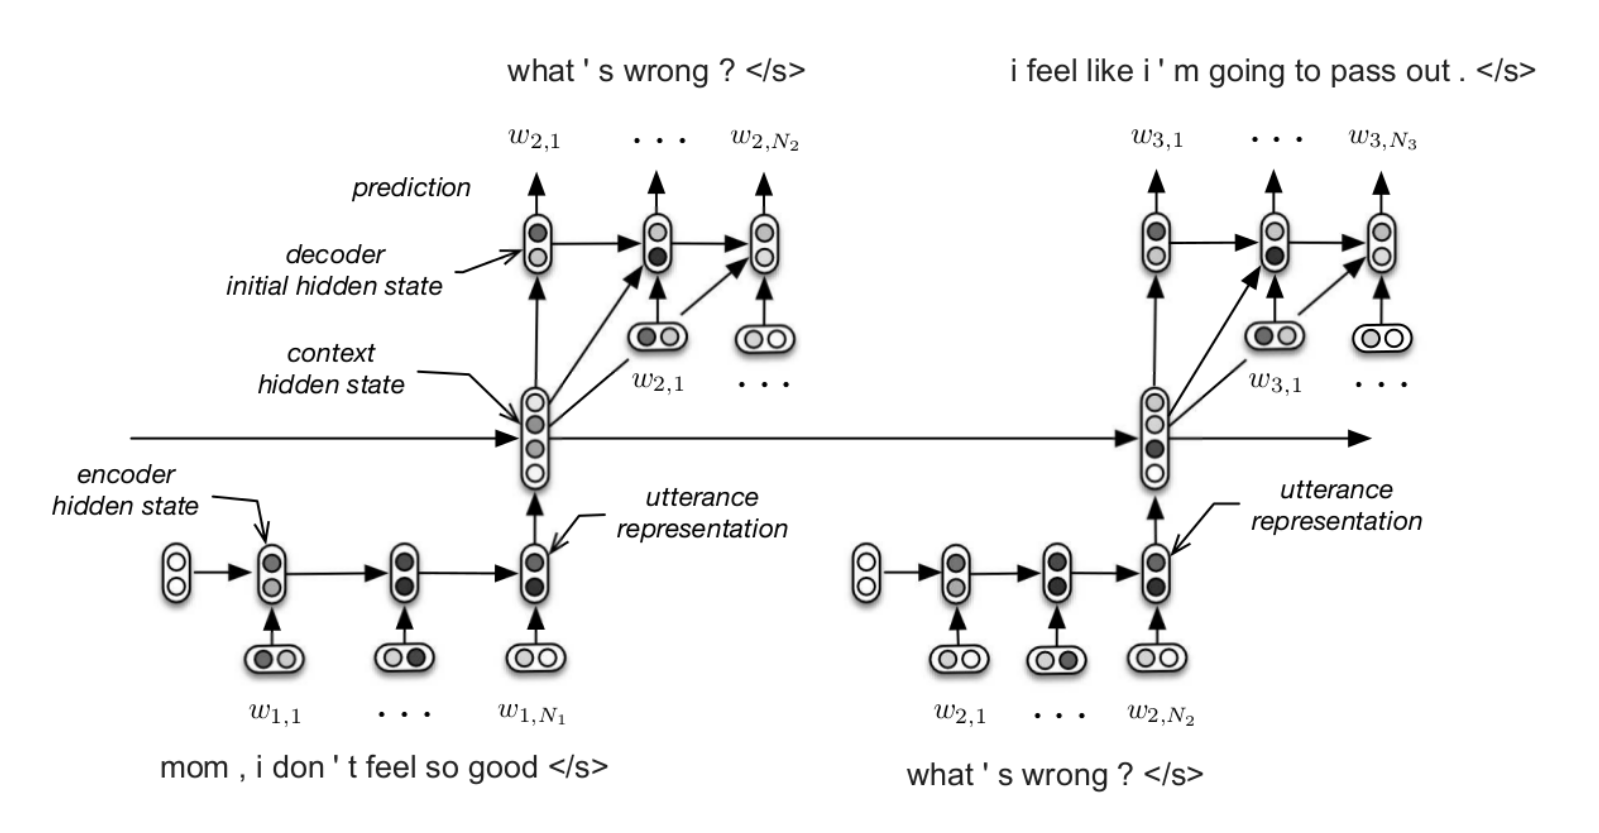
\includegraphics[width=\textwidth]{figure/HRED.png}
    \caption{HRED的计算图\upcite{HRED}}
    \label{fig:HRED_computation_graph}
\end{figure}


% ------------------ Decoding ------------------ %
\subsection{解码算法}\label{subsec:decode}
生成式模型仅仅定义了条件概率$p(Y|X)$,
在解码阶段,需要采用某种启发式搜索算法从概率分布中生成输出$Y$。
最简单的搜索算法是贪心搜索(Greedy Search):在每一时刻都输出条件概率最大的单词:
\begin{align}
    y_i = \argmax_{w \in V} p(w|y_1, y_2, \cdots, y_{i-1}, X)
\end{align}
因为各个$y_i$的概率都不是独立的,而是受之前输出的单词的影响,贪心搜索不能保证得到概率最大的输出序列。

随机取样(Random Sampling)
每生一步都从模型估计的全体词汇的离散概率分布中随机选取一个单词:
\begin{align}
    p(y_i = w) = p(w|y_1, y_2, \cdots, y_{i-1}, X), w \in V
\end{align}
Serban等人发现随机取样能避免单调响应的问题,并且能产生多样化的,
话题相关的输出\upcite{HRED},
但是Li等人指出随机取样会导致输出中出现语法错误\upcite{DiverseBeam}。

最为常用的方法是集束搜索(Beam Search),它在生成整个句子的过程中维护一个大小为$B$的列表,称为集束(Beam)。
算法开始时,集束初始化为模型生成的$B$个概率最高的单词。
在每一个时刻开始时,集束中都有$B$个部分生成的句子,它们称为候选$Y_c$。
在每一个时刻,算法对集束中的每一个候选都生成$B$个概率最大的下一个单词$w_{i+1, c}$,从而形成$B \times B$个部分生成的句子,
称为扩展的候选集。从扩展的候选集中,只保留前$B$个概率最大的句子。
算法不断迭代直到某些候选中产生了句子结束符号(End-of-Sentence,EOS),
算法将这些结束了的句子作为输出。
本质上,集束搜索是一种队列长度有限的宽度优先搜索
(Breath First Search)。

% ------ Diverse Beam -- %
为了增加模型输出的多样性,学者们提出了许多改进的解码算法。
Li等人提出了Diverse Beam算法,
在标准集束搜索中对来自相同父节点的候选加以惩罚,
即鼓励来自不同父节点的候选\upcite{DiverseBeam}。
% -- formula too complex to add -- %
% -- MMI -- %
Li等人还提出了以最大互信息(MMI)为目标函数的解码算法\upcite{MMI}。
本质上,他们训练了一个根据输入预测输出的正向模型(Forward Model)和
一个根据输出预测输入的反向模型(Backward Model),
再用反向模型的反向概率$p(Y|X)$对正向模型生成的候选集进行重新排序。
据此,他们提出了两种解码算法:MMI\_antiLM和MMI\_bidi,
分别如公式~\ref{eqn:MMI_antiLM}和公式~\ref{eqn:MMI_bidi}~所示:
\begin{align}
    MMI(S, T) &= \log \frac{p(S, T)}{p(S)p(T)} \label{eqn:MMI} \\
    \textit{MMI\_antiLM}(S, T) &= \log p(T|S) - \lambda \log p(T) \label{eqn:MMI_antiLM} \\
    \textit{MMI\_bidi}(S, T) &= (1 - \lambda) \log p(T|S) + \lambda \log p(S|T) \label{eqn:MMI_bidi}
\end{align}

% -- Stochastic Greedy Sampling -- %
Li等人还提出了随机贪心取样(Stochastic Greedy Sampling)算法
\upcite{Distill},
以求在随机取样和贪心搜索之间找到一个平衡点。
该算法只在条件概率最高的前$K$个候选单词中取样,
参数$K$控制了随机取样和贪心搜索之间的比例:
$K$越大,算法越接近随机取样,$K$越小,算法越接近贪心搜索。
这些改进的解码算法在不同程度上提高了响应的多样性。
% -- no formula found in paper -- %

% ------------------ Metrics ------------------ %
\section{自动化评价指标}\label{sec:automatic_metric}
\subsection{评价指标简介}\label{subsec:metrics_intro}
机器翻译领域已有大量和人类评价相关性较高的指标,例如
BLEU\upcite{BLEU},
NIST\upcite{NIST},
METEOR\upcite{METEOR},
BEER\upcite{beer},
CHRF\upcite{chrf},
TER\upcite{TER}等等。
然而,适用于开放领域的,面向闲聊的对话系统的指标要少得多;
在考察本领域对自动指标的使用情况之前,先对各种指标作一个简要介绍。

% --------------- BLEU ------------------ %
BLEU,Bilingual Evaluation Understudy\upcite{BLEU}是Papineni在2002年提出的,
用于机器翻译的自动评价指标。它是一个系统层面的评价指标,即评价一个系统在整个测试集上的性能。
BLEU指标只有一个参数$N$,表示要计算的各阶n-gram准确率的最大值;例如$N = 4$表示要计算1-gram到4-gram的准确率。
准确率指的是系统输出和参考输出之间的n-gram重叠数占系统输出总的n-gram的比例。
BLEU由在整个数据集上计算的各阶n-gram准确率的几何平均值(Geometric Mean)和简短惩罚系数(Brevity Penalty)相乘得到。
引入简短惩罚系数的原因是,较短的系统输出句子的准确率较高,需要矫正。
n-gram准确率的计算公式为:
\begin{align}
    p_n = \frac{
    \sum_{\mathcal{C} \in \{\textit{Candidates}\}
    \sum_{\textit{n-gram} \in \mathcal{C}}}
    \textit{Count}_{\textit{clip}}(\textit{n-gram})
    }{
    \sum_{\mathcal{C'} \in \{\textit{Candidates}\}}
    \sum_{\textit{n-gram}' \in \mathcal{C'}}
    \textit{Count}(\textit{n-gram}')
    }
\end{align}
Candidates为系统输出的句子集合,$\textit{Count}_{\textit{clip}}(\textit{n-gram})$为截断的n-gram共现数,
$\textit{Count}(\textit{n-gram}')$是Candidates中的总n-gram数。
简短惩罚系数BP的计算公式为
\begin{align}
    \textit{BP} =
    \begin{cases}
        \ 1 \ & \text{if} \  c > r \\
        \ e^{1 - r/c} \ & \text{if} \  c \leq r \\
    \end{cases}
\end{align}
其中$c$是模型输出句子的长度,$r$是参考输出句子的长度。
BLEU的最终公式为:
\begin{align}
    \textit{BLEU} = \textit{BP} \cdot \exp \left( \sum_{n=1}^N w_n \log p_n \right)
\end{align}
实际使用中一般取$N = 4$,$w_n = 1 / N$。
由于原始的BLEU容易在句子层面给出0分,人们提出了各种平滑处理\upcite{sBLEU-Smooth}。
本文在使用BLEU时也采用了一种平滑处理。

% ------------ ROUGE -------------- %
ROUGE,Recall-Oriented Understudy for Gisting Evaluation\upcite{ROUGE}是一种基于召回率的自动摘要领域的指标。
它有多个变形:ROUGE-N,ROUGE-L,ROUGE-W,ROUGE-S,以及ROUGE-SU,
分别使用了不同的计数单元(Counting Unit),如n-gram共现数、最长公共子序列(Longest Common Subsequence,LCS)和二元跳词(Skip-Bigram)等等。
这些指标的基础是信息检索领域常用的F-measure,即准确率和召回率的加权调和平均值:
\begin{align}
    \textit{F-measure} = \frac{(1 + \beta^2) RP}{R + \beta^2 P}
\end{align}
$\beta$控制准确率和召回率的相对重要性。
以下无特殊说明时,当指标是句子层面的时候,$n$是系统句子的长度,$m$是参考句子的长度;
当指标是摘要层面的时候,$n$是系统摘要的总单词数,$m$是参考摘要的总单词数。

ROUGE-N利用了n-gram共现数,其公式为:
\begin{align}
    \textit{ROUGE-N} = \frac{
    \sum_{S \in \{\textit{ReferenceSummaries}\}}
    \sum_{\textit{gram}_n \in S}
    \textit{Count}_\textit{matched}(\textit{gram}_n)
    }{
    \sum_{S \in \{\textit{ReferenceSummaries}\}}
    \sum_{\textit{gram}_n \in S}
    \textit{Count}(\textit{gram}_n)
    }
\end{align}
摘要层面的ROUGE-N具有相同的形式。

句子层面(Sentence Level)的ROUGE-L的公式为:
\begin{align}
    R_{lcs} &= \frac{\textit{LCS}(X, Y)}{m} \\
    P_{lcs} &= \frac{\textit{LCS}(X, Y)}{n} \\
    \textit{ROUGE-L} &= \frac{(1 + \beta^2) R_{lcs}P_{lcs}}
    {R_{lcs} + \beta^2 P_{lcs}}
\end{align}
$LCS$是计算两个序列的最长公共子序列的长度的函数。
摘要层面的ROUGE-L的公式为:
\begin{align}
    R_{lcs} &= \frac{\sum_{i=1}^\mu \textit{LCS}_\cup(r_i, C)}{m} \\
    P_{lcs} &= \frac{\sum_{i=1}^\mu \textit{LCS}_\cup(r_i, C)}{n} \\
    \textit{ROUGE-L} &= \frac{(1 + \beta^2) R_{lcs}P_{lcs}}{R_{lcs} + \beta^2 P_{lcs}}
\end{align}
$\mu$是系统输出的摘要句子的数量, $\textit{LCS}_\cup(r_i, C)$计算了参考句子$r_i$和候选摘要$C$(由多个句子组成)的LCS的并集。

句子层面的ROUGE-W的公式为:
\begin{align}
    R_{wlcs} &= f^{-1} \left( \frac{\textit{WLCS}(X, Y)}{f(m)} \right) \\
    P_{wlcs} &= f^{-1} \left( \frac{\textit{WLCS}(X, Y)}{f(n)} \right) \\
    \textit{ROUGE-W} &= \frac{(1 + \beta^2) R_{wlcs}P_{wlcs}}{R_{wlcs} + \beta^2 P_{wlcs}}
\end{align}
$\textit{WLCS}$是一个计算两个序列的加权LCS的算法,它奖励较长的连续的LCS。
摘要层面的ROUGE-W与摘要层面的ROUGE-L类似。

二元跳词是句子中顺序不变的一对单词,两个单词之间可以有任意数量的其他单词。
基于二元跳词的句子层面ROUGE-S定义为:
\begin{align}
    R_{skip2} &= \frac{\textit{SKIP2}(X, Y)}{C(m, 2)} \\
    P_{skip2} &= \frac{\textit{SKIP2}(X, Y)}{C(n, 2)} \\
    \textit{ROUGE-S} &= \frac{(1 + \beta^2) R_{skip2}P_{skip2}}{R_{skip2} + \beta^2 P_{skip2}}
\end{align}
$C(\cdot, \cdot)$为组合数。
摘要层面的ROUGE-S相当于把摘要看作首尾相连的句子来计算。
ROUGE-SU是ROUGE-S加入了Unigram的扩展。

% ----------------- METEOR ----------------- %
METEOR,Metric for Evaluation of Translation with Explicit ORdering
\upcite{METEOR}是针对BLEU的一些弱点提出的机器翻译的指标。
与BLEU相比,METEOR在句子水平上与人类评价有更好的相关性。
METEOR首先计算系统输出和参考输出之间的Unigram匹配,这些匹配由多个可配置的模块组成,
包括Exact,Porter-stem,WordNet-synonymy,分别表示严格匹配,Porter词根匹配和WordNet同义词匹配。
接着,METEOR在Unigram匹配上计算一个对齐,并得到基于Unigram匹配的准确率和召回率,进而得到二者的加权调和平均值:
\begin{align}
    \textit{Fmean} = \frac{10PR}{R + 9P}
\end{align}
METEOR还加入了对较短的n-gram匹配的惩罚系数:
\begin{align}
    \textit{Penalty} = 0.5 * \left( \frac{\#chunks}{\#unigrams\_matched} \right)
\end{align}
$\#unigrams\_matched$是所有匹配的Unigram的数量;
一个Unigram匹配越短,$\#chunks$就越大。
METEOR的最终公式为:
\begin{align}
    \textit{METEOR} = \textit{Fmean} * (1 - \textit{Penalty})
\end{align}

% --------- Perplexity ------------ %
困惑度(Perplexity,PPL)是一种衡量统计语言模型性能的指标。
一个模型的困惑度为$P$可以形象的表述为:
该模型在预测一个词的时候,平均需要从$P$个词中等可能的选出一个。
因此,困惑度越低,语言模型在选择一个词时就越不“困惑”。
困惑度的计算公式为:
\begin{align}
    \textit{PPL} = \exp(-\frac{1}{N} \sum_{i=1}^N \log p(x_i))
\end{align}
$N$是测试集的样本数,$x_i$是一个样本,在语言模型中它是一个句子,
在生成式模型中它是一对输入输出序列$(X, Y)$。
$p(x_i)$是模型估计的概率。
一个好的模型应该给测试集的样本估计较高的概率, 所以好的模型PPL较低。
实际在自然语言处理中使用的PPL还要除以文本中的总单词数,
得到平均每个词的困惑度(Perplexity per-word):
\begin{align}
    \textit{PPL-w} = \frac{1}{\#\textit{words}} \exp(-\frac{1}{N} \sum_{i=1}^N \log p(x_i))
\end{align}

% --------- embedding based ------------ %
词嵌入(Word Embedding)指标是一类建立在分布式假设
\upcite{distributed_hypothesis,Mathematical_structures_of_language}(Distributed Hypothesis)上,
用分布式语义(Distributed Semantic)来衡量两个句子的相似程度的指标,
常用于句子文本相似性(Sentence Textual Similarity)和学生输入自动打分\upcite{GreedyAndOptimal}等任务中。
这类指标一般用某种组合方式从单词的向量表示得到句子的向量表示,
再用余弦相似度(Cosine Similarity)测量两个句子向量的相似程度\upcite{VectorCompose}:
\begin{align}
    \text{cos}(x, y) = \frac{x\cdot y}
    {\left\| x \right\| \cdot \left\| y \right\|} \\
\end{align}
最常见组合方式是对单词向量取平均值,类似于词袋表示(Bag-of-Words),对应的指标就是向量平均值(Vector Average):
\begin{align}
    \bar{e_r} &= \frac{\sum_{w \in r} e_w}{|\sum_{w' \in r} e_{w'}|} \\
    \textit{Vector-Average} &= \cos(\bar{e_r}, \bar{e}_{\hat{r}})
\end{align}
$r$是参考输出,$\hat{r}$是系统输出,$w$是句子中的一个单词。

另外一种组合方式是向量极值(Vector Extrema),它把单词向量每个维度上的极端值作为句子向量在该维度上的值\upcite{Vector_Extrema}:
\begin{align}
    \text{extrema}(d_i) &=
    \begin{cases}
        \ \max d_i & \text{if}\ \max d_i \geq |\min d_i| \\
        \ \min d_i & \text{otherwise}
    \end{cases} \\
    e_r^{ex} &= [\text{extrema}(d_1), \cdots, \text{extrema}(d_n)] \\
    \textit{Vector-Extrema} &= \cos( e_r^{ex}, e_{\hat{r}}^{ex} )
\end{align}
$[\cdot, \cdot]$表示连接多个标量形成一个向量,
$e_r^{ex}$是参考输出的向量极值表示,$e_{\hat{r}}^{ex}$是系统输出的向量极值表示。

贪心匹配(Greedy Matching)
得名于边加权的二部图(Weighted Bipartite Graph)的最大匹配问题\upcite{GreedyAndOptimal}:
把两个句子的单词看做二部图的节点,任意两个节点之间有一条边,边的权重定义为两个单词的余弦相似度,一个匹配
定义为一对点,问如何构造一个匹配的集合,使其权重之和最大。贪心匹配给出了一种贪心算法:
\begin{align}
    G(r, \hat{r}) = \frac{
    \sum_{w \in r} \max_{\hat{w} \in \hat{r}} \cos(e_w, e_{\hat{w}})
    }{ |r| } \\
    \textit{Greedy-Matching} = \frac{
    G(r, \hat{r}) + G(\hat{r}, r)
    }{2}
\end{align}
除了上述三种组合方法外,还有很多其他方法\upcite{VectorCompose}。

% -------- Distinct-N ---------- %
Distinct-N是Li等人提出的衡量句子层面的n-gram多样性的指标\upcite{MMI}:
\begin{align}
    \textit{Distinct-N} = \frac{\#\textit{unique-ngrams}}{\#\textit{words}}
\end{align}

\subsection{评价指标使用情况}\label{subsec:metrics_usage}
生成式对话系统还没有公认的,与人类评价相关度较高的评价指标,
对话的研究者们很早就意识到了这一点\upcite{Ritter11,GoogleChatbot,Shang,HRED},
所以他们常常使用人类评价作为核心的评判标准,有时用一些指标来衡量模型某一方面的性质,
但很少把指标作为评价系统的主要手段。
此外,展示和对比不同模型的响应输出也是这个领域常见的分析手段,通常称为定性分析(Qualitative Analysis),比如
表~\ref{tab:qualitative_analysis}~展示了模型GoogleChatbot对哲学问题的响应。
\begin{table}[H]
    \centering
    \caption{定性分析的例子\upcite{GoogleChatbot}}
    \label{tab:qualitative_analysis}
    \begin{tabular}{ll}
        \textbf{Human:} & what is the purpose of life ? \\
        \textbf{Machine:} & to serve the greater good .\\
        \textbf{Human:} & what is the purpose of living ? \\
        \textbf{Machine:} & to live forever . \\
        \textbf{Human:} & what is the purpose of existence ? \\
        \textbf{Machine:} & to find out what happens when we get
        to the planet earth . \\
        \textbf{Human:} & where are you now ? \\
        \textbf{Machine:} & i' m in the middle of nowhere . \\
        \textbf{Human:} & what is the purpose of dying ? \\
        \textbf{Machine:} & to have a life . \\
        \textbf{Human:} & what is the purpose of being intelligent ? \\
        \textbf{Machine:} & to find out what it is . \\
        \textbf{Human:} & what is the purpose of emotions ? \\
        \textbf{Machine:} & i don' t know .
    \end{tabular}
\end{table}

% Ritter -- MT-chat
Ritter等人首次尝试了数据驱动的,面向闲聊的对话响应生成\upcite{Ritter11}。
因为不清楚面向任务的指标能不能用于评价生成式模型,他们就用了基于Amazon Mechanical Turk的人类评价。
他们利用人类评价的数据考察了BLEU在这方面的适用性,并发现系统的BLEU得分非常低,和人类评价的相关性也不是很高,
因此他们认为BLEU不能直接应用到本领域。


% Shang -- NRM
% We use abbreviation hereby. Remember to introduce their fullname before!
Shang等人在评价他们的NRM模型时分析了几种指标在本领域的适用性\upcite{Shang}。
他们认为BLEU并不适用,因为合理的响应的范围实在是太大了,参考响应不可能完全覆盖到;
而常用于语言模型的指标困惑度(Perplexity,PPL)也不适用,因为它不能测量响应的自然程度及其对消息的相关程度。
最后他们选择了人类评价。

% Sordoni -- DCGM-1-2
Sordoni在DCGM的评价时采用了BLEU和METEOR两种自动指标\upcite{DCGM}。
为了处理庞大而且多样的响应空间,他们用信息检索(Information Retrieval,IR)的方法从数据集中挖掘潜在的合理响应,
并让人类评估员对其合适度(Appropriateness)打分,
从而构造了一个多重参考评测集(Multiple-Responses Benchmark Dataset)。
在这样的评测集上,他们发现BLEU对系统的排名和人类评价非常一致。
这种构建多重响应测评集的方法也见于LSDSCC\upcite{LSDSCC}的测评集的构造方法,
以及DeltaBLEU\upcite{deltaBLEU}指标的设计思路。

% Serban -- HRED
Serban等人在HRED模型的评价中使用了困惑度和单词分类错误(Word Classification Error,WCE)\upcite{HRED}。
低的困惑度表示模型对数据的概率分布的拟合程度好。
Serban等人认为困惑度是适用的,因为在存在多个合理输出的情况下,困惑度总是衡量生成单一参考输出的概率,
这意味着它能可靠的衡量模型的质量。
WCE计算模型的输出中正确预测的单词占整个数据集单词数量的比例,
这里的“正确预测”要求单词在句子中的顺序也要正确,所以它是一个比困惑度更严苛的指标。
尽管使用了自动化指标,Serban等人指出:这些指标与他们想要衡量的语法正确度(Grammatical Correctness)
和语义连贯性(Semantic Coherence)之间的相关性并不明朗。
值得注意的是,他们并没有使用人类评价。

% Serban -- VHRED
Serban等人在VHRED模型的评价中主要使用了基于词嵌入的指标\upcite{VHRED}和人类评价。
Serban等人认为,虽然这些基于词嵌入的指标和人类评价的相关度不高,但是它们可以用于测量话题相似性(Topic Similarity),
也就是模型的输出和参考输出的语义内容是否相近。
模型的输出和参考输出可能没有n-gram重叠,但分布式语义可以给出非0的相似性。

% Google Chatbot
用Vinyals等人对\cite{GoogleChatbot}的评估结束本节:
他们使用了困惑度,定性分析和人类评价。
但是,他们认为这些测评方法都存在明显的弊端,而设计出能快速评价对话模型的好指标仍有待学界研究。


\section{生成式对话的数据集}\label{sec:public_dataset}
本领域在数据集的采集方面已经取得了很大进展,表~\ref{tab:dataset_list}~列举了一些常见数据集,
大规模是指对话数量在1M以上的,中等规模是指对话数量在50K--1M之间的\footnote{1K = 1024,1M = 1024 K,1G = 1024 M。}。
Sina Weibo Corpus是一个中文数据集,其他都是英文数据集。
Twitter相关的数据集由于隐私保护政策的原因,不能公开原始数据。
数据集\cite{supreme,wiki_pages,tennis_corpus,parliamentary,gone_awry,movie_dialogs_corpus,DailyDialog}都具有元信息,
如时间戳,对话双方身份信息等等。
数据集\cite{DailyDialog,LSDSCC,DCGM}有人类标注信息,如情感、话题和方面(Aspect)等。
元信息和人类标注信息提供了额外的表征,对构建更智能的对话系统很有帮助。
本文把注意力集中在三个数据集上:Ubuntu Dialogue Corpus,OpenSubtitles,LSDSCC,
因为它们分别代表了三个常见的对话领域,分别是:技术支持,电影字幕和在线论坛讨论。

\begin{table}[H]
    \centering
    \caption{数据集一览}
    \label{tab:dataset_list}
    \begin{tabular}{llll}
        \toprule
        名称 & 规模 & 领域 & 是否公开 \\
        \midrule
        Ubuntu Dialogue Corpus\upcite{ubuntu_corpus} & 大 & 技术支持 & 是 \\
        Twitter Corpus\upcite{Ritter11} & 大 & 短文本多领域闲聊 & 否 \\
        Twitter Triple Corpus\upcite{DCGM} & 大 & Twitter Corpus的扩展版本 & 否 \\
        OpenSubtitles\upcite{OPUS,opensub} & 大 & 电影字幕(Subtitles) & 是 \\
        LSDSCC\upcite{LSDSCC} & 中 & Reddit论坛电影板块 & 是 \\
        Supreme Court Corpus\upcite{supreme} & 中 & 美国高等法院辩论 & 是\\
        Wikipedia Talk Pages Corpus\upcite{wiki_pages} & 中 & 维基百科编辑者在线讨论 & 是 \\
        Tennis Corpus\upcite{tennis_corpus} & 中 & 网球比赛赛后新闻发布会 & 是 \\
        Parliament Corpus\upcite{parliamentary} & 中 & 国会讨论 & 是 \\
        Conversations Gone Awry Corpus\upcite{gone_awry} & 中 & 维基百科讨论页面吵架集锦 & 是 \\
        Movie Dialogs Corpus\upcite{movie_dialogs_corpus} & 中 & 电影对白 & 是 \\
        Movie-DiC\upcite{Movie-DiC} & 中 & IMSDB电影对白 & 否 \\
        MovieTriples\upcite{HRED} & 中 & Movie-DiC的扩展版本 & 否 \\
        SubTle\upcite{Luke_SubTle} & 中 & 电影字幕 & 否 \\
        DailyDialog\upcite{DailyDialog} & 中 & 日常对话 & 是 \\
        Sina Weibo Corpus\upcite{weibo} & 中 & 新浪微博短文本闲聊 & 是 \\
        \bottomrule
    \end{tabular}
\end{table}

% --------- Ubuntu ---------- %
Ubuntu Dialogue Corpus是Lowe等人从Freenode IRC网络的Ubuntu板块的聊天日志\footnote{https://irclogs.ubuntu.com/}
中获取的技术性两人多轮对话。这个数据集中包含了大量技术符号,比如路径、命令、URL,还有笔误(Typo),缩写(Abbreviation)和俚语(Slang)。
它的对话数量多达930,000(接近1M),庞大的数据量为数据驱动的模型提供了极佳的试验场。
它的多轮特性为模型提供了更长的上下文,有助于能利用多轮对话的模型生成更有意义的响应。

% --------- OpenSubtitles -------- %
OpenSubtitles是The Open Parallel Corpus,OPUS项目的一部分。
它是从一个人们可以自由上传和下载电影字幕的网站\footnote{http://www.opensubtitles.org}的数据库中获取的,
庞大而充满噪音的开放领域数据集。
它的对话数量达到了80M。
由于OPUS的目的是收集机器翻译所用到的双语文库(Parallel Corpus),OpenSubtitles也是一个用于机器翻译的双语文库,
它里面并没有对话数据集所需要的轮换信息(Turn-Taking),而且也没有区分旁白、独白和对白。
Sordoni等人在\cite{GoogleChatbot}中把OpenSubtitles用到对话领域,
他们把相邻的两个句子视为消息和响应,并且每一个句子既是消息又是响应。
Li等人在\cite{MMI,persona,Future,DiverseBeam,
Distill,deep_RL,Adversarial}中对OpenSubtitles也采用了类似办法。
尽管充满噪音,OpenSubtitles仍然是目前最大规模的电影字幕数据集。

% --------- LSDSCC ------------- %
LSDSCC,A Large Scale Domain-Specific Conversational Corpus是一个单一领域的单轮对话数据集\upcite{LSDSCC}。
有研究认为,单一领域和专注的话题有助于模型规避单调的响应。
它有738,095个对话,词汇表比较大,达到了50K。
作者从Reddit的电影板块\footnote{https://www.reddit.com/r/datasets}中获取了原始数据,
设计了一套尽可能保留语料信息的清理程序,还使用人类评价员对消息和响应的相关度进行评价,
最终得到一个高质量的信息-响应对(Query-Response Pair)文库。
在构建测试集方面,作者用类似\cite{DCGM}的IR方法构建了一个多重参考评测集。
他们还进一步让人类评价员对一个消息的所有响应进行分类,并
基于这个测试集提出了三个面向多样性的评价指标,不过我们并未使用。

\section{本章小结}\label{sec:rw_conclusion}
本章从模型、指标和数据集三个方面回顾了本领域的研究成果和现存问题。
在模型方面,基于Seq2Seq的对话系统能够直接生成响应,能端对端的训练,减少写死的规则(Hard Written Rules),
能从大量语料数据中自动学习语言规律,能利用话题和情感等多种表征,具有巨大的优越性。
然而,这类系统也有弊端,比如无法准确控制生成的内容,偏向于生成单调的响应,
没有人格一致性等等。

在指标方面,对话系统的指标还不能像机器翻译的指标那样准确的评价对话系统。
可能最大的问题就是,如何提高指标和人类评价的相关性。
导致这个困境的核心原因可能是对话的响应具有固有的语义多样性,
这个事实可能导致两个结果:1. 用机器翻译的表征,比如单词层面的n-gram,字符层面的n-gram,
对齐等等,无法有效捕捉语义层面的信息。
2. 单纯使用衡量相似性的指标无法捕捉多样性的维度,从而与人类评价不符。

在数据集方面,本领域已经积累了各种领域(Domain)的数据,从技术性问答、社交媒体闲聊,到电影对白和字幕等等。
既有大规模的数据集,也有中等规模,但是具有元信息或者人类标注信息的数据集。
因为数据集的增多,一些数据集在领域上出现了重合,比如Movie Dialogs Corpus,MovieTriples和Movie-DiC都是
电影对白领域;OpenSubtitles和SubTle都是电影字幕领域,Twitter Corpus和Sina Weibo Corpus都是短文本闲聊等等。
尽管人类标注是对话文本的重要补充,但是由于其代价的高昂,所得的数据量往往比较少;
另一方面,元信息是一类在数据采集过程中,伴随对话文本同时获得的描述性信息,比如对话者的性别(Gender)和角色(Character)。
相比与人类标注,元信息更容易获取,规模不受限制。
并且,人类标注和元信息都有助于模型生成更加多样和连贯的响应\upcite{persona,Topic_Aware,ECM}。
因此,数据集的收集过程应该充分保留原始数据中的元信息; 对话系统应该充分利用元信息。
同时,还应该发展从对话文本中无监督的提取元信息的方法。

尽管本领域取得了丰硕的成果,我们应该持续关注并且不断探索上述难题的解决方案。
本文就试图在一个多维度的设定下,研究不同的评价指标和不同的模型以及数据集之间的交互关系。
